%-----------------------------------------------------------------------------%
\chapter{\babTiga}
%-----------------------------------------------------------------------------%

%-----------------------------------------------------------------------------%
\section{Desain Sistem}
%-----------------------------------------------------------------------------%

Untuk dapat menghasilkan program sesuai tujuan, maka perlu dilakukan desain mengenai sistem secara keseluruhan. Sesuai dengan tujuan dari program yang akan menghubungkan antara Zotonic dan \textit{web service} yang dihasilkan oleh ABS \textit{mircoservice} maka diperlukan sebuah \textit{script} pada Zotonic untuk menghubungkan keduanya.

\begin{figure}
	\centering
	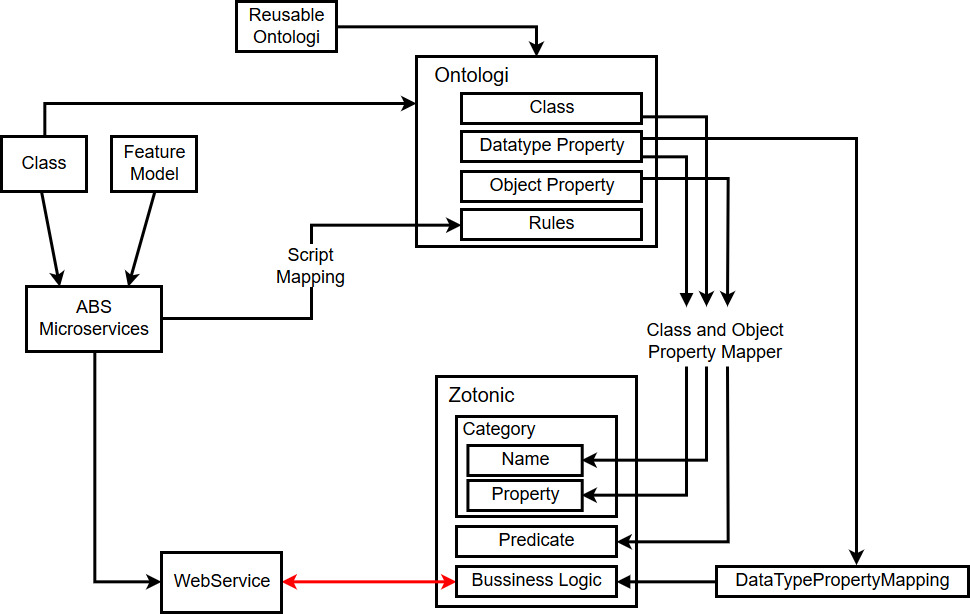
\includegraphics[width=1\textwidth]
		{pics/skripsiRoadmap.jpg}
	\caption{Desain sistem secara keseluruhan}
	\label{fig:skripsiroadmap}
\end{figure}
\vspace{-0.8cm}

%-----------------------------------------------------------------------------%
\section{Desain \f{Bussiness Logic}}
%-----------------------------------------------------------------------------%
Beberapa perintah yang dapat digunakan untuk mengubah tampilan adalah: 
\begin{itemize}
	\item \bslash f \\
		Merupakan alias untuk perintah \bslash textit, contoh 
		\f{contoh hasil tulisan}.
	\item \bslash bi \\
		\bi{Contoh hasil tulisan}.
	\item \bslash bo \\
		\bo{Contoh hasil tulisan}.
	\item \bslash code \\ 
		\code{Contoh hasil tulisan}.
\end{itemize}

%-----------------------------------------------------------------------------%
\section{Desain \f{Rules}}
%-----------------------------------------------------------------------------%
Beberapa perintah yang dapat digunakan untuk mengubah tampilan adalah: 
\begin{itemize}
	\item \bslash f \\
		Merupakan alias untuk perintah \bslash textit, contoh 
		\f{contoh hasil tulisan}.
	\item \bslash bi \\
		\bi{Contoh hasil tulisan}.
	\item \bslash bo \\
		\bo{Contoh hasil tulisan}.
	\item \bslash code \\ 
		\code{Contoh hasil tulisan}.
\end{itemize}
